\chapter{Consigna 1: filtro pasa alto pasivo RLC}
\label{chap:consigna1}

\section{Diseño del Filtro}

Se adopta la topología de la Figura~\ref{fig:circuito}: la resistencia $R$ y el capacitor $C$ en serie con
la entrada, y el inductor $L$ en paralelo sobre la salida. La elección se fundamenta en que, con esta
disposición, la resistencia interna del generador $R_g$ queda en serie con $R$ y se incorpora al diseño
como una resistencia total $R_t = R_g + R$, de modo que una resistencia de generador comparativamente baja
no modifica apreciablemente el comportamiento del filtro.

\begin{figure}[!ht]
  \centering
  \begin{subfigure}[t]{0.48\textwidth}
    \centering
    \begin{tikzpicture}[american]
  \draw (0,0) to[short, o-] (0.4,0)
        to[R, l=$R$] (2.2,0)
        to[C, l=$C$] (4,0)
        to[short, -o] (5.5,0);
  \draw (4,0) to[L, l=$L$, *-*] (4,-2.5);
  \draw (0,-2.5) to[short, o-o] (5.5,-2.5);
  \draw (4,-2.5) node[ground]{};
  \draw (0,0) to[open, v=$v_i(t)$] (0,-2.5);
  \draw (5.5,0) to[open, v=$v_o(t)$] (5.5,-2.5);
\end{tikzpicture}

    \caption{Circuito en el dominio del tiempo.}
    \label{crkt:pasa-alto}
  \end{subfigure}
  \hfill
  \begin{subfigure}[t]{0.48\textwidth}
    \centering
    \begin{tikzpicture}[american]
  \draw (0,0) to[short, o-] (0.4,0)
        to[generic, l=$R$, i=$I(s)$] (2.2,0)
        to[generic, l=\tiny$\frac{1}{sC}$] (4,0)
        to[short, -o] (5.5,0);
  \draw (4,0) to[generic, l=$sL$, *-*] (4,-2.5);
  \draw (0,-2.5) to[short, o-o] (5.5,-2.5);
  \draw (4,-2.5) node[ground]{};
  \draw (0,0) to[open, v=$V_i(s)$] (0,-2.5);
  \draw (5.5,0) to[open, v=$V_o(s)$] (5.5,-2.5);
\end{tikzpicture}

    \caption{Modelo de impedancias en el dominio de Laplace.}
    \label{crkt:laplace}
  \end{subfigure}
  \caption{Filtro pasa alto pasivo RLC de segundo orden.}
  \label{fig:circuito}
\end{figure}

\section{Función de transferencia}

Analizando el circuito de la Figura~\ref{crkt:laplace}, la corriente de malla es

\begin{equation}
  I(s) = \frac{V_i(s)}{R + \dfrac{1}{sC} + sL} = \frac{sC}{s^2 LC + sRC + 1}\, V_i(s),
  \label{eq:corriente}
\end{equation}

y la tensión de salida es la caída sobre el inductor, $V_o(s) = sL\, I(s)$. Reemplazando la
ecuación~\eqref{eq:corriente} y dividiendo numerador y denominador por $LC$ se obtiene la función de
transferencia en términos de los componentes:

\begin{equation}
  H(s) = \frac{V_o(s)}{V_i(s)} = \frac{s^2 LC}{s^2 LC + sRC + 1}
       = \frac{s^2}{s^2 + s\,\dfrac{R}{L} + \dfrac{1}{LC}}.
  \label{eq:tf-componentes}
\end{equation}

La ecuación~\eqref{eq:tf-componentes} presenta un cero doble en el origen y dos polos dados por las raíces
del polinomio característico, lo que confirma el comportamiento pasa alto de segundo orden: para $s \to 0$
la ganancia tiende a cero y para $s \to \infty$ tiende a la unidad.

\section{Forma canónica y ecuaciones de diseño}

La forma canónica de un pasa alto de segundo orden es

\begin{equation}
  H(s) = \frac{s^2}{s^2 + \dfrac{\omega_0}{Q}\, s + \omega_0^2},
  \label{eq:tf-canonica}
\end{equation}

donde $\omega_0$ es la pulsación natural y $Q$ el factor de calidad. Comparando término a término las
ecuaciones~\eqref{eq:tf-componentes} y~\eqref{eq:tf-canonica} resulta el sistema

\begin{gather*}
  \omega_0^2 = \frac{1}{LC}, \qquad \frac{\omega_0}{Q} = \frac{R}{L},
\end{gather*}

de donde, fijando $R$ como parámetro libre, se despejan los valores de los componentes:

\begin{equation}
  L = \frac{R\,Q}{\omega_0}, \qquad C = \frac{1}{\omega_0\, R\, Q}.
  \label{eq:diseno-LC}
\end{equation}

\subsection{Relación entre la frecuencia de corte y la pulsación natural}

La pulsación natural $\omega_0$ coincide con la pulsación de corte $\omega_c$ (atenuación de
\qty{-3}{\decibel}) únicamente cuando $Q = 1/\sqrt{2}$ (respuesta de Butterworth). Para cualquier otro valor
de $Q$ es necesario introducir una constante de corrección $K$ tal que $\omega_0 = K\,\omega_c$. Su
expresión se obtiene imponiendo la condición de \qty{-3}{\decibel} sobre el módulo de la
ecuación~\eqref{eq:tf-canonica}. Definiendo $x = \omega/\omega_0$,

\begin{gather*}
  |H(jx)|^2 = \frac{x^4}{\left(1 - x^2\right)^2 + \dfrac{x^2}{Q^2}} = \frac{1}{2}
  \;\Longrightarrow\;
  x^4 + \left(2 - \frac{1}{Q^2}\right) x^2 - 1 = 0,
\end{gather*}

cuya única solución positiva, llamando $a = 1 - \dfrac{1}{2Q^2}$, es $x_c^2 = -a + \sqrt{a^2 + 1}$. Como
$K = \omega_0/\omega_c = 1/x_c$, racionalizando se obtiene

\begin{equation}
  K = \sqrt{\left(1 - \frac{1}{2Q^2}\right) + \sqrt{\left(1 - \frac{1}{2Q^2}\right)^2 + 1}}.
  \label{eq:factor-K}
\end{equation}

Reemplazando $\omega_0 = 2\pi f_c K$ en la ecuación~\eqref{eq:diseno-LC}, las ecuaciones de diseño
quedan expresadas directamente en función de los datos del problema:

\begin{equation}
  L = \frac{R\,Q}{2\pi f_c\, K}, \qquad C = \frac{1}{2\pi f_c\, K\, Q\, R}.
  \label{eq:diseno-final}
\end{equation}

\subsection{Factor de amortiguamiento}

Expresando el denominador de la ecuación~\eqref{eq:tf-canonica} en la forma estándar de los sistemas de
segundo orden, $s^2 + 2\xi\omega_0 s + \omega_0^2$, el factor de amortiguamiento resulta

\begin{equation}
  \xi = \frac{1}{2Q},
  \label{eq:xi}
\end{equation}

y su valor determina el tipo de amortiguamiento: sobreamortiguado si $\xi > 1$ (raíces reales y distintas),
críticamente amortiguado si $\xi = 1$ (raíz real doble) y subamortiguado si $\xi < 1$ (raíces complejas
conjugadas).

\section{Elección de la resistencia}

Se elige $R = \qty{100}{\ohm}$ como compromiso entre dos criterios: un valor suficientemente alto para que
la resistencia interna del generador (típicamente \qty{50}{\ohm} o menor) no altere de manera significativa
el factor de calidad del filtro, y suficientemente bajo para que, según la ecuación~\eqref{eq:diseno-final},
no resulten valores de inductancia excesivamente elevados.

\section{Valores de los componentes}

Aplicando las ecuaciones~\eqref{eq:factor-K}, \eqref{eq:diseno-final} y~\eqref{eq:xi} con
$f_c = \qty{400}{\hertz}$ y $R = \qty{100}{\ohm}$ se obtienen los valores de la
Tabla~\ref{tab:componentes}. A modo de ejemplo, para $Q = \num{0.25}$:

\begin{gather*}
  K = \sqrt{\left(1 - \frac{1}{2 \cdot \num{0.25}^2}\right)
      + \sqrt{\left(1 - \frac{1}{2 \cdot \num{0.25}^2}\right)^2 + 1}} = \num{0.2666}, \\[4pt]
  L = \frac{\qty{100}{\ohm} \cdot \num{0.25}}{2\pi \cdot \qty{400}{\hertz} \cdot \num{0.2666}}
    = \qty{37.31}{\milli\henry}, \qquad
  C = \frac{1}{2\pi \cdot \qty{400}{\hertz} \cdot \num{0.2666} \cdot \num{0.25} \cdot \qty{100}{\ohm}}
    = \qty{59.70}{\micro\farad}.
\end{gather*}

\begin{gather*}
  K = \sqrt{\left(1 - \frac{1}{2 \cdot \num{0.75}^2}\right)
      + \sqrt{\left(1 - \frac{1}{2 \cdot \num{0.75}^2}\right)^2 + 1}} = \num{1.057}, \\[4pt]
  L = \frac{\qty{100}{\ohm} \cdot \num{0.75}}{2\pi \cdot \qty{400}{\hertz} \cdot \num{1.057}}
    = \qty{28.23}{\milli\henry}, \qquad
  C = \frac{1}{2\pi \cdot \qty{400}{\hertz} \cdot \num{1.057} \cdot \num{0.75} \cdot \qty{100}{\ohm}}
    = \qty{5.02}{\micro\farad}.
\end{gather*}

\begin{table}[H]
  \centering
  \begin{tabular}{|c|c|c|c|c|c|c|}
    \hline
    $Q$ & $K$ & $\omega_0$ [\unit{\radian\per\second}] & $f_0$ [\unit{\hertz}] & $L$ & $C$ & $\xi$ \\
    \hline
    \num{0.25} & \num{0.2666} & \num{670.0}  & \num{106.6} & \qty{37.31}{\milli\henry}
               & \qty{59.70}{\micro\farad} & \num{2.000} \\
    \num{0.75} & \num{1.0570} & \num{2656.5} & \num{422.8} & \qty{28.23}{\milli\henry}
               & \qty{5.02}{\micro\farad}  & \num{0.667} \\
    \hline
  \end{tabular}
  \caption{Constante de corrección, pulsación natural, componentes y factor de amortiguamiento de cada diseño.}
  \label{tab:componentes}
\end{table}

\section{Análisis para $Q = \num{0.25}$}

\subsection{Función de transferencia}

Con $R = \qty{100}{\ohm}$, $L = \qty{37.31}{\milli\henry}$ y $C = \qty{59.70}{\micro\farad}$, los
coeficientes de la ecuación~\eqref{eq:tf-componentes} resultan

\begin{gather*}
  \frac{R}{L} = \frac{\qty{100}{\ohm}}{\qty{37.31}{\milli\henry}} = \num{2680.25}, \qquad
  \frac{1}{LC} = \frac{1}{\qty{37.31}{\milli\henry} \cdot \qty{59.70}{\micro\farad}} = \num{448952.5},
\end{gather*}

por lo que la función de transferencia del filtro es

\begin{equation}
  H_1(s) = \frac{s^2}{s^2 + \num{2680.25}\, s + \num{448952.5}}
         = \frac{s^2}{\left(s + \num{179.53}\right)\left(s + \num{2500.72}\right)}.
  \label{eq:tf-q025}
\end{equation}

\subsection{Raíces y lugar de raíces}

El polinomio característico tiene discriminante positivo
($\num{2680.25}^2 - 4 \cdot \num{448952.5} > 0$), de modo que sus raíces son reales y distintas:

\begin{gather*}
  s_1 = \num{-179.53}\ \unit{\radian\per\second}, \qquad
  s_2 = \num{-2500.72}\ \unit{\radian\per\second},
\end{gather*}

a las que se suma el cero doble en el origen. La Figura~\ref{fig:polos-q025} muestra su ubicación en el
plano complejo: ambos polos se encuentran sobre el semieje real negativo, uno de ellos
($s_1$, equivalente a \qty{28.6}{\hertz}) mucho más cercano al origen que el otro
($s_2$, equivalente a \qty{398}{\hertz}). El polo $s_2$ es el que fija en la práctica la frecuencia de corte,
mientras que $s_1$ es el polo dominante de la respuesta temporal.

\begin{figure}[!ht]
  \centering
  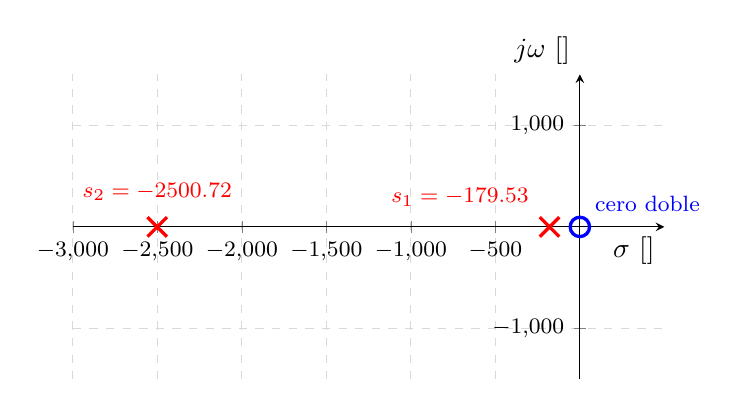
\begin{tikzpicture}
  \begin{axis}[
    width=0.75\textwidth, height=0.45\textwidth,
    axis lines=middle,
    xlabel={$\sigma$ [\unit{\radian\per\second}]},
    ylabel={$j\omega$ [\unit{\radian\per\second}]},
    xlabel style={at={(ticklabel* cs:1)}, anchor=north east},
    ylabel style={at={(ticklabel* cs:1)}, anchor=south east},
    xmin=-3000, xmax=500, ymin=-1500, ymax=1500,
    xtick={-3000,-2500,-2000,-1500,-1000,-500},
    ytick={-1000,1000},
    grid=both, grid style={gray!30, dashed},
    tick label style={font=\footnotesize},
    clip=false,
  ]
    \addplot[only marks, mark=x, mark size=5pt, very thick, red]
      coordinates {(-2500.72,0) (-179.53,0)};
    \addplot[only marks, mark=o, mark size=3.5pt, very thick, blue] coordinates {(0,0)};
    \node[above=6pt, red, font=\footnotesize] at (axis cs:-2500.72,0) {$s_2 = \num{-2500.72}$};
    \node[above left=4pt, red, font=\footnotesize] at (axis cs:-179.53,0) {$s_1 = \num{-179.53}$};
    \node[above right=2pt, blue, font=\footnotesize] at (axis cs:0,0) {cero doble};
  \end{axis}
\end{tikzpicture}

  \caption{Ubicación de polos y ceros de $H_1(s)$ en el plano complejo.}
  \label{fig:polos-q025}
\end{figure}

\subsection{Factor de amortiguamiento}

De la ecuación~\eqref{eq:xi},

\begin{equation}
  \xi = \frac{1}{2Q} = \frac{1}{2 \cdot \num{0.25}} = 2,
  \label{eq:xi-q025}
\end{equation}

valor mayor que la unidad y coherente con las dos raíces reales distintas halladas. La constante de
corrección de la frecuencia de corte para este caso es $K = \num{0.2666}$, lo que indica que la pulsación
natural $\omega_0 = \qty{670.0}{\radian\per\second}$ se encuentra muy por debajo de la de corte.

\subsection{Respuesta temporal}

Se analiza la respuesta ante un escalón unitario, $v_i(t) = u(t)$, cuya transformada es
$V_i(s) = 1/s$. La salida en el dominio de Laplace es entonces

\begin{equation}
  V_o(s) = H_1(s)\, V_i(s)
         = \frac{s}{\left(s + \num{179.53}\right)\left(s + \num{2500.72}\right)}
         = \frac{A}{s + \num{179.53}} + \frac{B}{s + \num{2500.72}}.
  \label{eq:vo-q025}
\end{equation}

Igualando numeradores, $A\left(s + \num{2500.72}\right) + B\left(s + \num{179.53}\right) = s$, lo que
conduce al sistema $A + B = 1$ y $\num{2500.72}\,A + \num{179.53}\,B = 0$. Resolviendo:

\begin{gather*}
  A = \frac{\num{-179.53}}{\num{2500.72} - \num{179.53}} = \num{-0.07734}, \qquad
  B = \frac{\num{2500.72}}{\num{2500.72} - \num{179.53}} = \num{1.07734}.
\end{gather*}

Antitransformando término a término se obtiene la respuesta temporal

\begin{equation}
  v_o(t) = \left(\num{1.07734}\, e^{-\num{2500.72}\, t} - \num{0.07734}\, e^{-\num{179.53}\, t}\right) u(t),
  \label{eq:vo-t-q025}
\end{equation}

que se grafica en la Figura~\ref{fig:escalon-q025}. En $t = 0^+$ la salida reproduce íntegramente el salto
de entrada ($v_o(0^+) = A + B = 1$), ya que el capacitor se comporta como un cortocircuito y el inductor
como un circuito abierto frente al flanco. Luego la salida decae hacia cero: el término rápido se extingue
en pocas décimas de milisegundo y el término lento, de signo negativo, provoca un pequeño paso por valores
negativos antes de alcanzar el valor final.

\begin{figure}[!ht]
  \centering
  \begin{tikzpicture}
  \begin{axis}[
    name=principal,
    width=0.9\textwidth, height=0.55\textwidth,
    xlabel={$t$ [\unit{\milli\second}]}, ylabel={Tensión [\unit{\volt}]},
    xmin=0, xmax=12, ymin=-0.1, ymax=1.1,
    grid=both, grid style={gray!30, dashed},
    legend pos=north east, legend cell align=left, legend style={font=\footnotesize},
    tick label style={font=\footnotesize},
    samples=400, domain=0:12, no marks,
  ]
    \addplot[gray, thick, dotted] {1};
    \addlegendentry{$v_i(t)$ (escalón unitario)}
    \addplot[blue, very thick] {1.07734*exp(-2.50072*x) - 0.07734*exp(-0.17953*x)};
    \addlegendentry{$v_o(t)$ para $Q = \num{0.25}$}
    \addplot[red, dashed] {0.02};
    \addlegendentry{banda de $\pm\qty{2}{\percent}$}
    \addplot[red, dashed, forget plot] {-0.02};
    \draw[dashed, gray] (axis cs:7.53,-0.1) -- (axis cs:7.53,0.08);
  \end{axis}
  % detalle ampliado de la zona del subpico
  \begin{axis}[
    at={(principal.north east)}, anchor=north east, xshift=-0.6cm, yshift=-2.0cm,
    width=0.5\textwidth, height=0.28\textwidth,
    xmin=0, xmax=12, ymin=-0.07, ymax=0.04,
    ytick={-0.06,-0.04,-0.02,0,0.02},
    scaled y ticks=false,
    yticklabel style={/pgf/number format/fixed, /pgf/number format/precision=2},
    grid=both, grid style={gray!30, dashed},
    tick label style={font=\scriptsize},
    axis background/.style={fill=white},
    samples=400, domain=0:12, no marks,
  ]
    \addplot[blue, very thick] {1.07734*exp(-2.50072*x) - 0.07734*exp(-0.17953*x)};
    \addplot[red, dashed] {0.02};
    \addplot[red, dashed] {-0.02};
    \addplot[only marks, mark=*, mark size=1.5pt, black] coordinates {(2.269,-0.0478)};
    \node[below right=1pt, font=\scriptsize] at (axis cs:2.269,-0.0478)
      {subpico \qty{-4.8}{\percent} en $t = \qty{2.27}{\milli\second}$};
    \draw[dashed, gray] (axis cs:7.53,-0.07) -- (axis cs:7.53,0.04)
      node[pos=0.72, right, font=\scriptsize, black] {$t_s = \qty{7.53}{\milli\second}$};
    \node[anchor=north west, font=\scriptsize\itshape] at (rel axis cs:0.02,0.98) {detalle};
  \end{axis}
\end{tikzpicture}

  \caption{Respuesta al escalón unitario del filtro con $Q = \num{0.25}$.}
  \label{fig:escalon-q025}
\end{figure}

\subsection{Parámetros de la respuesta temporal}

Dado que la respuesta al escalón de un filtro pasa alto parte del valor del salto y evoluciona hacia cero,
los parámetros clásicos de los sistemas de segundo orden se adaptan de la siguiente manera: el tiempo de
crecimiento se reemplaza por el tiempo de caída entre el \qty{90}{\percent} y el \qty{10}{\percent} del
salto inicial; el sobrepico se mide como la máxima excursión por debajo del valor final (subpico),
referida al salto inicial; y el tiempo de establecimiento es el instante a partir del cual la salida
permanece dentro de una banda de $\pm\qty{2}{\percent}$ del salto alrededor del valor final. Los valores
medidos sobre la ecuación~\eqref{eq:vo-t-q025} se resumen en la Tabla~\ref{tab:parametros-q025}.

\begin{table}[!ht]
  \centering
  \begin{tabular}{|l|c|}
    \hline
    Parámetro & Valor \\
    \hline
    Valor inicial $v_o(0^+)$                              & \qty{1}{\volt} \\
    Tiempo de caída (\qty{90}{\percent} a \qty{10}{\percent}) & \qty{0.70}{\milli\second} \\
    Subpico máximo                                        & \qty{-4.8}{\percent} \\
    Instante del subpico                                  & \qty{2.27}{\milli\second} \\
    Tiempo de establecimiento (\qty{2}{\percent})         & \qty{7.53}{\milli\second} \\
    Constante de tiempo dominante $\tau_1 = 1/|s_1|$      & \qty{5.57}{\milli\second} \\
    \hline
  \end{tabular}
  \caption{Parámetros de la respuesta al escalón para $Q = \num{0.25}$.}
  \label{tab:parametros-q025}
\end{table}

El tiempo de establecimiento queda determinado casi exclusivamente por el polo dominante: a partir de la
ecuación~\eqref{eq:vo-t-q025}, despreciando el término rápido, la salida ingresa definitivamente en la
banda del \qty{2}{\percent} cuando $\num{0.07734}\, e^{-t/\tau_1} = \num{0.02}$, es decir, en
$t_s = \tau_1 \ln\left(\num{0.07734}/\num{0.02}\right) = \qty{7.53}{\milli\second}$, en coincidencia con el
valor medido.

\subsection{Tipo de amortiguamiento}

Con $\xi = 2 > 1$ y dos raíces reales distintas, el filtro es sobreamortiguado. La respuesta no presenta
oscilaciones: la salida decae de forma monótona hasta un único subpico de muy baja amplitud
(\qty{-4.8}{\percent}) y luego retorna lentamente a cero, gobernada por la constante de tiempo del polo
más cercano al origen.

\section{Análisis para $Q = \num{0.75}$}

\subsection{Función de transferencia}

Con $R = \qty{100}{\ohm}$, $L = \qty{28.23}{\milli\henry}$ y $C = \qty{5.02}{\micro\farad}$, los
coeficientes de la ecuación~\eqref{eq:tf-componentes} resultan

\begin{gather*}
  \frac{R}{L} = \frac{\qty{100}{\ohm}}{\qty{28.23}{\milli\henry}} = \num{3542.33}, \qquad
  \frac{1}{LC} = \frac{1}{\qty{28.23}{\milli\henry} \cdot \qty{5.02}{\micro\farad}} = \num{7056436},
\end{gather*}

y la función de transferencia del filtro es

\begin{equation}
  H_2(s) = \frac{s^2}{s^2 + \num{3542.33}\, s + \num{7056436}}
         = \frac{s^2}{\left(s + \num{1771.17} + j\,\num{1979.75}\right)
                       \left(s + \num{1771.17} - j\,\num{1979.75}\right)}.
  \label{eq:tf-q075}
\end{equation}

\subsection{Raíces y lugar de raíces}

En este caso el discriminante del polinomio característico es negativo
($\num{3542.33}^2 - 4 \cdot \num{7056436} < 0$) y las raíces son complejas conjugadas:

\begin{gather*}
  s_{1,2} = -\sigma \pm j\,\omega_d = \num{-1771.17} \pm j\,\num{1979.75}\ \unit{\radian\per\second},
\end{gather*}

con parte real $\sigma = \xi\omega_0 = \num{1771.17}$ y pulsación amortiguada
$\omega_d = \omega_0\sqrt{1 - \xi^2} = \num{1979.75}$. Junto con el cero doble en el origen, su ubicación
se muestra en la Figura~\ref{fig:polos-q075}. Los polos se encuentran sobre una circunferencia de radio
$\omega_0 = \qty{2656.4}{\radian\per\second}$ y forman con el semieje real negativo un ángulo
$\theta = \arccos\xi = \qty{48.2}{\degree}$.

\begin{figure}[!ht]
  \centering
  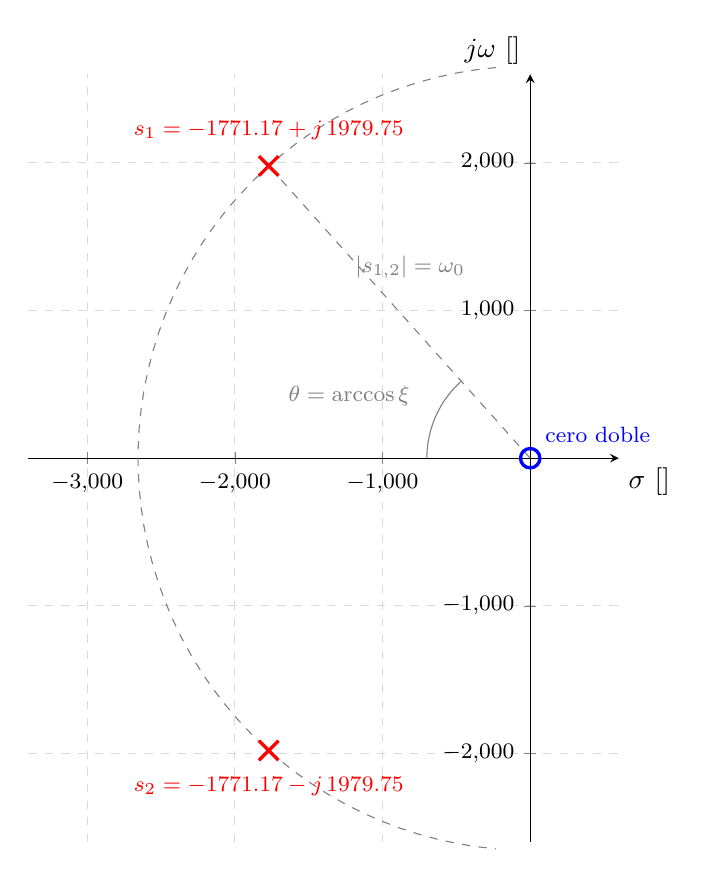
\begin{tikzpicture}
  \begin{axis}[
    % escala igual en ambos ejes: 4000 x 5200 rad/s sobre 7,5 cm x 9,75 cm
    scale only axis, width=7.5cm, height=9.75cm,
    axis lines=middle,
    xlabel={$\sigma$ [\unit{\radian\per\second}]},
    ylabel={$j\omega$ [\unit{\radian\per\second}]},
    xlabel style={at={(ticklabel* cs:1)}, anchor=north west},
    ylabel style={at={(ticklabel* cs:1)}, anchor=south east},
    xmin=-3400, xmax=600, ymin=-2600, ymax=2600,
    xtick={-3000,-2000,-1000},
    ytick={-2000,-1000,1000,2000},
    grid=both, grid style={gray!30, dashed},
    tick label style={font=\footnotesize},
    clip=false,
  ]
    % circunferencia de radio omega_0 sobre la que se ubican los polos
    \addplot[domain=95:265, samples=60, dashed, gray, no marks] ({2656.4*cos(x)}, {2656.4*sin(x)});
    \addplot[dashed, gray, no marks] coordinates {(0,0) (-1771.17,1979.75)};
    \addplot[domain=131.8:180, samples=20, gray, no marks] ({700*cos(x)}, {700*sin(x)});
    \addplot[only marks, mark=x, mark size=5pt, very thick, red]
      coordinates {(-1771.17,1979.75) (-1771.17,-1979.75)};
    \addplot[only marks, mark=o, mark size=3.5pt, very thick, blue] coordinates {(0,0)};
    \node[above=6pt, red, font=\footnotesize] at (axis cs:-1771.17,1979.75)
      {$s_1 = \num{-1771.17} + j\,\num{1979.75}$};
    \node[below=6pt, red, font=\footnotesize] at (axis cs:-1771.17,-1979.75)
      {$s_2 = \num{-1771.17} - j\,\num{1979.75}$};
    \node[above right=2pt, blue, font=\footnotesize] at (axis cs:0,0) {cero doble};
    \node[gray, font=\footnotesize, anchor=south west] at (axis cs:-1250,1150) {$|s_{1,2}| = \omega_0$};
    \node[gray, font=\footnotesize, anchor=east] at (axis cs:-750,420) {$\theta = \arccos\xi$};
  \end{axis}
\end{tikzpicture}

  \caption{Ubicación de polos y ceros de $H_2(s)$ en el plano complejo.}
  \label{fig:polos-q075}
\end{figure}

\subsection{Factor de amortiguamiento}

De la ecuación~\eqref{eq:xi},

\begin{equation}
  \xi = \frac{1}{2Q} = \frac{1}{2 \cdot \num{0.75}} = \num{0.667},
  \label{eq:xi-q075}
\end{equation}

valor menor que la unidad, en concordancia con el par de raíces complejas conjugadas. La constante de
corrección vale $K = \num{1.0570}$, es decir, la pulsación natural
$\omega_0 = \qty{2656.5}{\radian\per\second}$ queda apenas por encima de la pulsación de corte
($\qty{2513.3}{\radian\per\second}$).

\subsection{Respuesta temporal}

Ante un escalón unitario, $V_i(s) = 1/s$, la salida en el dominio de Laplace es

\begin{equation}
  V_o(s) = H_2(s)\, V_i(s)
         = \frac{s}{\left(s + \num{1771.17}\right)^2 + \num{1979.75}^2}.
  \label{eq:vo-q075}
\end{equation}

Para antitransformar se suma y resta $\sigma$ en el numerador, de modo de expresar la función como
combinación de las transformadas de $e^{-\sigma t}\cos(\omega_d t)$ y $e^{-\sigma t}\sin(\omega_d t)$:

\begin{gather*}
  V_o(s) = \frac{s + \num{1771.17}}{\left(s + \num{1771.17}\right)^2 + \num{1979.75}^2}
         - \frac{\num{1771.17}}{\num{1979.75}} \cdot
           \frac{\num{1979.75}}{\left(s + \num{1771.17}\right)^2 + \num{1979.75}^2}, \\[4pt]
  \frac{\sigma}{\omega_d} = \frac{\num{1771.17}}{\num{1979.75}} = \num{0.8946}.
\end{gather*}

La respuesta temporal resulta entonces

\begin{equation}
  v_o(t) = e^{-\num{1771.17}\, t}
           \left[\cos\left(\num{1979.75}\, t\right) - \num{0.8946}\, \sin\left(\num{1979.75}\, t\right)\right] u(t),
  \label{eq:vo-t-q075}
\end{equation}


La Figura~\ref{fig:escalon-q075} muestra la respuesta junto con
su envolvente exponencial. Nuevamente $v_o(0^+) = 1$, pero ahora la salida cruza por cero, alcanza un
subpico apreciable y oscila con pulsación $\omega_d$ dentro de la envolvente
$\pm\frac{\omega_0}{\omega_d} e^{-\sigma t}$ hasta extinguirse.

\begin{figure}[!ht]
  \centering
  \begin{tikzpicture}
  \begin{axis}[
    width=0.9\textwidth, height=0.5\textwidth,
    xlabel={$t$ [\unit{\milli\second}]}, ylabel={Tensión [\unit{\volt}]},
    xmin=0, xmax=4, ymin=-0.35, ymax=1.1,
    grid=both, grid style={gray!30, dashed},
    legend pos=north east, legend cell align=left, legend style={font=\footnotesize},
    tick label style={font=\footnotesize},
    samples=400, domain=0:4, no marks,
  ]
    \addplot[gray, thick, dotted] {1};
    \addlegendentry{$v_i(t)$ (escalón unitario)}
    \addplot[blue, very thick]
      {exp(-1.77117*x)*(cos(deg(1.97975*x)) - 0.8946*sin(deg(1.97975*x)))};
    \addlegendentry{$v_o(t)$ para $Q = \num{0.75}$}
    \addplot[orange, dashed, thick] {1.3416*exp(-1.77117*x)};
    \addlegendentry{envolvente $\pm\frac{\omega_0}{\omega_d}e^{-\sigma t}$}
    \addplot[orange, dashed, thick, forget plot] {-1.3416*exp(-1.77117*x)};
    \addplot[red, dashed] {0.02};
    \addlegendentry{banda de $\pm\qty{2}{\percent}$}
    \addplot[red, dashed, forget plot] {-0.02};
    \addplot[only marks, mark=*, mark size=1.8pt, black, forget plot] coordinates {(0.850,-0.222)};
    \node[below right=2pt, font=\footnotesize] at (axis cs:0.850,-0.222)
      {subpico \qty{-22.2}{\percent} en $t = \qty{0.85}{\milli\second}$};
    \addplot[only marks, mark=*, mark size=1.8pt, black, forget plot] coordinates {(0.425,0)};
    \node[above right=2pt, font=\footnotesize] at (axis cs:0.425,0) {$t = \qty{0.425}{\milli\second}$};
    \draw[dashed, gray] (axis cs:1.82,-0.35) -- (axis cs:1.82,0.5)
      node[pos=1, above, font=\footnotesize, black] {$t_s = \qty{1.82}{\milli\second}$};
  \end{axis}
\end{tikzpicture}

  \caption{Respuesta al escalón unitario del filtro con $Q = \num{0.75}$.}
  \label{fig:escalon-q075}
\end{figure}

\subsection{Parámetros de la respuesta temporal}

Con el mismo criterio de medición adoptado para $Q = \num{0.25}$, los parámetros obtenidos sobre la
ecuación~\eqref{eq:vo-t-q075} se listan en la Tabla~\ref{tab:parametros-q075}. El primer cruce por cero se
obtiene de forma analítica igualando a cero el corchete de la ecuación~\eqref{eq:vo-t-q075}:
$\tan(\omega_d t) = \omega_d/\sigma$, de donde
$t_0 = \arctan(\num{1.1178})/\num{1979.75} = \qty{0.425}{\milli\second}$.

\begin{table}[H]
  \centering
  \begin{tabular}{|l|c|}
    \hline
    Parámetro & Valor \\
    \hline
    Valor inicial $v_o(0^+)$                                  & \qty{1}{\volt} \\
    Tiempo de caída (\qty{90}{\percent} a \qty{10}{\percent}) & \qty{0.33}{\milli\second} \\
    Primer cruce por cero                                     & \qty{0.425}{\milli\second} \\
    Subpico máximo                                            & \qty{-22.2}{\percent} \\
    Instante del subpico                                      & \qty{0.85}{\milli\second} \\
    Tiempo de establecimiento (\qty{2}{\percent})             & \qty{1.82}{\milli\second} \\
    Pulsación amortiguada $\omega_d$                          & \qty{1979.75}{\radian\per\second} \\
    Período de la oscilación $T_d = 2\pi/\omega_d$            & \qty{3.17}{\milli\second} \\
    \hline
  \end{tabular}
  \caption{Parámetros de la respuesta al escalón para $Q = \num{0.75}$.}
  \label{tab:parametros-q075}
\end{table}

\subsection{Tipo de amortiguamiento}

Con $\xi = \num{0.667} < 1$ y raíces complejas conjugadas, el filtro es subamortiguado. La respuesta es
oscilatoria amortiguada: la salida cruza por cero, presenta un subpico del \qty{22.2}{\percent} del salto
y continúa oscilando con período $T_d = \qty{3.17}{\milli\second}$, aunque la fuerte atenuación de la
envolvente ($\sigma = \num{1771.17}$) hace que solo el primer semiciclo negativo sea apreciable y que la
salida se establezca en menos de \qty{2}{\milli\second}.

\section{Comparación de los diseños y tipos de amortiguamiento}

\subsection{Comparación de las respuestas obtenidas}

La Figura~\ref{fig:escalon-comparacion} superpone las respuestas al escalón de ambos filtros y la
Tabla~\ref{tab:comparacion} resume sus parámetros. Si bien ambos diseños comparten la misma frecuencia de
corte, el comportamiento transitorio es claramente distinto: el filtro sobreamortiguado tarda unas cuatro
veces más en establecerse, pero su excursión por debajo del valor final es casi cinco veces menor que la
del filtro subamortiguado.

\begin{figure}[!ht]
  \centering
  \begin{tikzpicture}
  \begin{axis}[
    width=0.9\textwidth, height=0.5\textwidth,
    xlabel={$t$ [\unit{\milli\second}]}, ylabel={$v_o(t)$ [\unit{\volt}]},
    xmin=0, xmax=8, ymin=-0.3, ymax=1.05,
    grid=both, grid style={gray!30, dashed},
    legend pos=north east, legend cell align=left, legend style={font=\footnotesize},
    tick label style={font=\footnotesize},
    samples=400, domain=0:8, no marks,
  ]
    \addplot[blue, very thick] {1.07734*exp(-2.50072*x) - 0.07734*exp(-0.17953*x)};
    \addlegendentry{$Q = \num{0.25}$ ($\xi = 2$, sobreamortiguado)}
    \addplot[red!80!black, very thick]
      {exp(-1.77117*x)*(cos(deg(1.97975*x)) - 0.8946*sin(deg(1.97975*x)))};
    \addlegendentry{$Q = \num{0.75}$ ($\xi = \num{0.667}$, subamortiguado)}
    \addplot[gray, dashed] {0.02};
    \addlegendentry{banda de $\pm\qty{2}{\percent}$}
    \addplot[gray, dashed, forget plot] {-0.02};
  \end{axis}
\end{tikzpicture}

  \caption{Respuestas al escalón unitario para ambos valores de $Q$.}
  \label{fig:escalon-comparacion}
\end{figure}

\begin{table}[!ht]
  \centering
  \begin{tabular}{|l|c|c|}
    \hline
    Parámetro & $Q = \num{0.25}$ & $Q = \num{0.75}$ \\
    \hline
    Factor de amortiguamiento $\xi$                          & \num{2.000} & \num{0.667} \\
    Tipo de amortiguamiento                                   & sobreamortiguado & subamortiguado \\
    Raíces [\unit{\radian\per\second}]                        & $\num{-179.53}$ ; $\num{-2500.72}$
                                                              & $\num{-1771.17} \pm j\,\num{1979.75}$ \\
    Tiempo de caída (\qty{90}{\percent} a \qty{10}{\percent}) & \qty{0.70}{\milli\second}
                                                              & \qty{0.33}{\milli\second} \\
    Subpico máximo                                            & \qty{-4.8}{\percent} & \qty{-22.2}{\percent} \\
    Tiempo de establecimiento (\qty{2}{\percent})             & \qty{7.53}{\milli\second} & \qty{1.82}{\milli\second} \\
    Inductancia $L$                                           & \qty{37.31}{\milli\henry} & \qty{28.23}{\milli\henry} \\
    Capacidad $C$                                             & \qty{59.70}{\micro\farad} & \qty{5.02}{\micro\farad} \\
    \hline
  \end{tabular}
  \caption{Comparación de los parámetros de ambos diseños.}
  \label{tab:comparacion}
\end{table}

La diferencia en el comportamiento transitorio tiene su contraparte en la respuesta en frecuencia
(Figura~\ref{fig:bode-comparacion}). En el filtro sobreamortiguado los dos polos reales se encuentran muy
separados (\qty{28.6}{\hertz} y \qty{398}{\hertz}), de manera que entre ambas frecuencias la pendiente de
atenuación es de solo \qty{20}{\decibel} por década y la transición hacia la banda de rechazo es gradual.
En el filtro subamortiguado los polos complejos actúan en conjunto alrededor de $f_0 = \qty{422.8}{\hertz}$ y
la pendiente de \qty{40}{\decibel} por década se alcanza inmediatamente por debajo de la frecuencia de corte.
Como ejemplo, una señal de \qty{100}{\hertz} (dos octavas por debajo de $f_c$) se atenúa
\qty{12.6}{\decibel} con $Q = \num{0.25}$ y \qty{25.0}{\decibel} con $Q = \num{0.75}$. Para $Q = \num{0.75}$
el pico de resonancia es despreciable ($Q/\sqrt{1 - 1/(4Q^2)} = \num{1.006}$, equivalente a
\qty{0.05}{\decibel}), por lo que la banda de paso se mantiene prácticamente plana.

\begin{figure}[!ht]
  \centering
  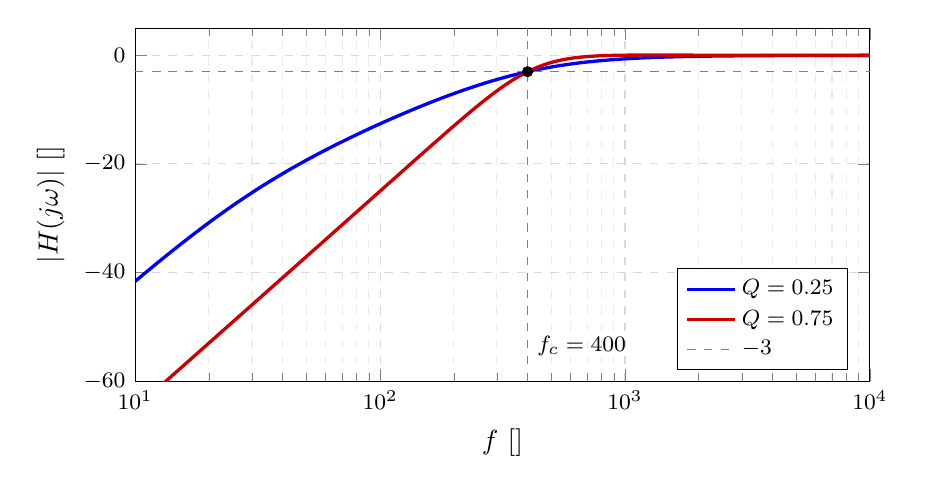
\begin{tikzpicture}
  \begin{semilogxaxis}[
    width=0.9\textwidth, height=0.5\textwidth,
    xlabel={$f$ [\unit{\hertz}]}, ylabel={$|H(j\omega)|$ [\unit{\decibel}]},
    xmin=10, xmax=10000, ymin=-60, ymax=5,
    grid=both, grid style={gray!30, dashed},
    minor grid style={gray!15, dashed},
    legend pos=south east, legend cell align=left, legend style={font=\footnotesize},
    tick label style={font=\footnotesize},
    samples=150, domain=10:10000, no marks,
  ]
    \addplot[blue, very thick]
      {20*log10((2*pi*x)^2 / sqrt((670.04^2 - (2*pi*x)^2)^2 + (670.04*2*pi*x/0.25)^2))};
    \addlegendentry{$Q = \num{0.25}$}
    \addplot[red!80!black, very thick]
      {20*log10((2*pi*x)^2 / sqrt((2656.40^2 - (2*pi*x)^2)^2 + (2656.40*2*pi*x/0.75)^2))};
    \addlegendentry{$Q = \num{0.75}$}
    \addplot[gray, dashed] {-3.01};
    \addlegendentry{$\qty{-3}{\decibel}$}
    \draw[dashed, gray] (axis cs:400,-60) -- (axis cs:400,5)
      node[pos=0.1, right, font=\footnotesize, black] {$f_c = \qty{400}{\hertz}$};
    \addplot[only marks, mark=*, mark size=1.8pt, black, forget plot] coordinates {(400,-3.01)};
  \end{semilogxaxis}
\end{tikzpicture}

  \caption{Módulo de la respuesta en frecuencia de ambos filtros.}
  \label{fig:bode-comparacion}
\end{figure}

\subsection{Ventajas de cada tipo de amortiguamiento}

\subsubsection{Sobreamortiguado ($\xi > 1$)}

\begin{itemize}
  \item La respuesta es no oscilatoria: no hay \emph{ringing} y el subpico es muy pequeño (en este diseño,
        del \qty{4.8}{\percent}), lo que resulta ventajoso cuando la señal filtrada alimenta etapas sensibles
        a excursiones de signo contrario (comparadores, detectores de nivel, etapas con limitación de
        excursión).
  \item El comportamiento es robusto frente a la tolerancia de los componentes: una variación de $L$, $C$ o
        de la resistencia de generador desplaza los polos sobre el eje real sin riesgo de que la respuesta
        se vuelva oscilatoria.
  \item La respuesta queda gobernada por una única constante de tiempo dominante, lo que simplifica su
        análisis y su predicción.
  \item Como contrapartida, el tiempo de establecimiento es largo y la transición entre la banda de paso y
        la de rechazo es poco selectiva; además, por ser $\omega_0$ mucho menor que $\omega_c$, se requieren
        componentes de mayor valor (en este caso un capacitor de \qty{59.70}{\micro\farad}).
\end{itemize}

\subsubsection{Críticamente amortiguado ($\xi = 1$)}

\begin{itemize}
  \item Corresponde a $Q = \num{0.5}$ y constituye el límite entre los dos casos anteriores: es la respuesta
        más rápida que puede obtenerse sin que aparezcan oscilaciones.
  \item Es la elección habitual cuando se busca minimizar el tiempo de establecimiento con la condición
        estricta de no sobrepasar el valor final.
  \item Su desventaja es que resulta un punto de diseño frágil: cualquier dispersión de componentes lo
        convierte en uno de los otros dos tipos.
\end{itemize}

\subsubsection{Subamortiguado ($\xi < 1$)}

\begin{itemize}
  \item Es el tipo de respuesta más rápida: en este diseño el tiempo de caída se reduce a la mitad y el
        tiempo de establecimiento a la cuarta parte respecto del caso sobreamortiguado.
  \item La respuesta en frecuencia es más selectiva: la pendiente de \qty{40}{\decibel} por década se
        alcanza inmediatamente por debajo de $f_c$ y la banda de paso es más plana, de modo que se filtran
        mejor las componentes cercanas a la frecuencia de corte.
  \item Al ser $\omega_0 \approx \omega_c$, los componentes resultan de menor valor (en este caso un
        capacitor de \qty{5.02}{\micro\farad}), lo que facilita su implementación con componentes no
        electrolíticos y de mejor tolerancia.
  \item La desventaja es la aparición de oscilaciones y de un subpico importante (\qty{22.2}{\percent}), que
        crece a medida que $Q$ aumenta; para valores de $Q$ superiores a $1/\sqrt{2}$ aparece además un pico
        de resonancia en la banda de paso que, para $Q = \num{0.75}$, todavía es despreciable.
\end{itemize}
